\documentclass[10pt,twocolumn]{article}

%% ── Packages ──────────────────────────────────────────────────────────────────
\usepackage[margin=1in]{geometry}
\usepackage{amsmath,amssymb}
\usepackage{graphicx}
\usepackage{booktabs}
\usepackage{hyperref}
\usepackage{xcolor}
\usepackage{multirow}
\usepackage{microtype}
\usepackage{caption}
\usepackage{subcaption}
\usepackage{algorithm}
\usepackage{algpseudocode}
\usepackage{enumitem}
\setlist{itemsep=2pt,parsep=0pt}

%% ── Metadata ──────────────────────────────────────────────────────────────────
\title{\textbf{Quantum-Inspired Tensor-Network Compression of OpenVLA-7B}\\[4pt]
  \large Global Quantum + AI Challenge 2026 --- VW Group Enterprise Track\\
  Sub-track: Compression $|$ Domain: Robotics}
\author{Benjamin Brumm}
\date{July 2026}

%% ── Macros ────────────────────────────────────────────────────────────────────
\newcommand{\chi}{\ensuremath{\mathcal{X}}}
\newcommand{\PENDING}[1]{\textcolor{red}{\textbf{[PENDING: #1]}}}
\newcommand{\placeholder}[1]{\textcolor{red}{\textbf{#1}}}

\hypersetup{
  colorlinks=true,
  linkcolor=blue,
  citecolor=blue,
  urlcolor=blue,
}

\begin{document}
\maketitle

%% ─────────────────────────────────────────────────────────────────────────────
\begin{abstract}
We present a quantum-inspired tensor-network (TN) compression pipeline for
OpenVLA-7B \cite{kim2024openvla}, a 7.54\,B-parameter vision-language-action model
for robot manipulation. Following the CompactifAI methodology \cite{tomut2024compactifai},
we decompose the 6.48\,B-parameter LLM backbone's linear-layer weight matrices into
Matrix Product State (MPS) representations using GPU-accelerated SVD
(\texttt{torch.linalg.svd}), sweeping bond dimension $\chi \in \{16,32,64,128\}$.
At $\chi=64$ the LLM backbone is compressed by $44.5\times$ (per layer), reducing
total parameter count from 7.54\,B to approximately 1.20\,B (6.3$\times$ overall).
We evaluate action-prediction fidelity against a FP16 baseline on the
\texttt{lerobot/toto} dataset (7-DoF manipulation, proxy for the Open X-Embodiment
bridge split \cite{open_x_embodiment_2023}), and demonstrate the compressed model
driving a dm\_control MuJoCo humanoid. A PennyLane circuit-depth analysis shows the
$\chi=16$ regime is feasible on near-term NISQ hardware (total CNOT depth $\approx87$).
\end{abstract}

%% ─────────────────────────────────────────────────────────────────────────────
\section{Introduction}

Large vision-language-action (VLA) models like OpenVLA-7B promise generalised robot
control from language and camera observations, but their 7--13\,B parameter count
makes on-device deployment impractical. The standard mitigation---INT8 quantisation
via \texttt{bitsandbytes}---achieves 2--4$\times$ compression with modest accuracy
loss, but hits a practical ceiling: further bit-width reduction degrades performance
sharply and is unsupported on several GPU generations (e.g.\ P100/sm\_60); recent
NVIDIA FP4 work \cite{nvfp4} pushes this ceiling further on Blackwell GPUs but
remains hardware-generation locked.

Tensor-network (TN) methods from quantum many-body physics offer a complementary
path. Matrix Product States (MPS) and Matrix Product Operators (MPO) represent
high-dimensional tensors as chains of low-rank cores whose expressive power is
controlled by a single hyperparameter---the bond dimension $\chi$. The number of
parameters scales as $O(\chi^2 d)$ rather than $O(mn)$, yielding tunable
compression at any target ratio. The CompactifAI work \cite{tomut2024compactifai}
showed this is viable for large language models; we extend it to the multimodal
action-prediction setting of OpenVLA-7B.

Concurrent VLA architectures such as $\pi_0$ \cite{black2024pi0} push toward
generalised robot control via flow-matching policies at similar scale.
Related work on structured classical compression includes SQAP-VLA and similar
pruning-plus-quantisation pipelines, which offer strong baselines but share the
quantisation ceiling. Our approach trades heavier offline compute (SVD sweep) for a
potentially better compression-accuracy frontier at high ratios---we do not claim
outright superiority, but aim to map the frontier across $\chi$ values and identify
which regime is practically useful.

%% ─────────────────────────────────────────────────────────────────────────────
\section{Method: MPS/MPO Compression}

\subsection{Theoretical Foundation}

A weight matrix $W \in \mathbb{R}^{m \times n}$ can be reshaped into a
higher-order tensor $\mathcal{W} \in \mathbb{R}^{d_1 \times d_2 \times \cdots \times d_k}$
(with $\prod_i d_i = mn$). An MPS decomposition expresses this as a contraction of
$k$ core tensors:
\[
  \mathcal{W}_{i_1 i_2 \cdots i_k}
  \;=\;
  \sum_{\alpha_1,\ldots,\alpha_{k-1}}
    A^{(1)}_{i_1,\alpha_1}
    A^{(2)}_{\alpha_1,i_2,\alpha_2}
    \cdots
    A^{(k)}_{i_k,\alpha_{k-1}}
\]
where each bond index $\alpha_j$ runs over $\chi$ values. The total parameter
count of the MPS representation is $O(\chi^2 \cdot \sum_j d_j)$, compared to
$O(mn)$ for the dense matrix. The approximation is obtained by truncating singular
values in a sequence of SVDs along the chain.

This is the quantum-inspired analog of the MPO used in density-matrix renormalisation
group (DMRG) algorithms for quantum many-body ground states \cite{liu2024provable}.
The bond dimension $\chi$ directly corresponds to the entanglement cut-off in
quantum information theory: a state with limited bipartite entanglement is exactly
representable by an MPS with finite $\chi$.

\subsection{Algorithm}

We target the attention and feed-forward linear layers of the LLM backbone:
\texttt{q\_proj}, \texttt{k\_proj}, \texttt{v\_proj}, \texttt{o\_proj},
\texttt{gate\_proj}, \texttt{up\_proj}, \texttt{down\_proj} across all 32
transformer layers (224 total, 217 successfully compressed). Vision-encoder
(SigLIP) layers are excluded in the primary configuration; Section~\ref{sec:ablation}
compares LLM-only vs.\ full compression.

Algorithm~\ref{alg:mps} summarises the compression loop.
For an $m \times n$ weight matrix we use $k=4$ sites with physical dimensions
chosen to minimise the approximation error subject to $\prod_j d_j = mn$.
Reconstruction contracts the cores in-place and replaces the original
\texttt{nn.Linear} module with a FP16 \texttt{nn.Linear} containing the
reconstructed weight. All SVDs run on the GPU via \texttt{torch.linalg.svd}
(cuSOLVER backend), with reconstruction performed on CPU to avoid exhausting the
P100's $\sim$100\,MiB headroom post model-load.

\begin{algorithm}[t]
\small
\caption{MPS weight compression}\label{alg:mps}
\begin{algorithmic}[1]
\Require Weight $W \in \mathbb{R}^{m \times n}$, bond dimension $\chi$, sites $k=4$
\State Reshape $W$ into $\mathcal{W} \in \mathbb{R}^{d_1 \times d_2 \times d_3 \times d_4}$
\For{$j = 1, \ldots, k-1$}
  \State $\mathcal{W} \leftarrow$ reshape to matrix $M \in \mathbb{R}^{(\prod_{i \leq j} d_i \cdot \chi_\text{prev}) \times (\prod_{i > j} d_i)}$
  \State $U, \Sigma, V^\top \leftarrow$ \texttt{torch.linalg.svd}$(M)$, truncate to $\chi$
  \State Store core $A^{(j)} \leftarrow U[:, :\chi]$; set $\mathcal{W} \leftarrow \text{diag}(\Sigma[:\chi]) \cdot V^\top[:\chi,:]$
\EndFor
\State Store final core $A^{(k)} \leftarrow \mathcal{W}$
\State $\hat{W} \leftarrow$ contract$(A^{(1)}, \ldots, A^{(k)})$ and reshape to $m \times n$
\State Replace \texttt{nn.Linear} weight with $\hat{W}$ (FP16)
\end{algorithmic}
\end{algorithm}

\subsection{Quantum-Inspired Justification}

The MPS structure is directly borrowed from quantum information: an $n$-qubit
quantum state with bounded bipartite entanglement across any cut is exactly
representable as an MPS with finite $\chi$. The mathematical equivalence means that
the TN compression of a weight matrix is isomorphic to preparing a quantum state
with a structured circuit of depth $O(\chi^2)$ per bond---a connection made concrete
in our PennyLane feasibility analysis (Appendix~\ref{app:pennylane}).

Unlike INT8 quantisation, which applies a fixed bit-width uniformly, MPS compression
is adaptive: singular values that fall below the truncation threshold contribute
negligibly to the network's function, so the information-theoretic compression is
guided by the structure of the weight matrices rather than imposed externally. This
constitutes the quantum-inspired advantage claimed in~\S5.5.

%% ─────────────────────────────────────────────────────────────────────────────
\section{Experimental Setup}

\subsection{Model}

We use OpenVLA-7B \cite{kim2024openvla} (\texttt{openvla/openvla-7b}), a
Prismatic-VLM architecture combining a SigLIP vision encoder with a
Vicuna-v1.5/LLaMA-2 language backbone (7.54\,B parameters total; 6.48\,B in the
LLM backbone layers we target).

\textbf{License note.} The OpenVLA-7B model \emph{code} is MIT-licensed.
The \emph{weights} are governed by the \textbf{LLaMA-2 Community License
(non-commercial research use only)}. All experiments in this work are strictly
research-use. Users wishing to reproduce results must accept the LLaMA-2 license
on HuggingFace Hub before downloading weights.

\textbf{Baseline.} The accepted baseline for this sub-track is INT8 quantisation
via \texttt{bitsandbytes}. On our evaluation hardware (Tesla P100, sm\_60),
\texttt{bitsandbytes} INT8 is not supported (minimum requirement: sm\_75). We
therefore use a FP16 (half-precision) floating-point baseline, which gives a fair
upper bound on model quality; all $\Delta$-accuracy numbers are relative to this
FP16 reference. The hardware constraint and this choice are documented in
\texttt{results/baseline\_metrics.json} and in Appendix~\ref{app:resources}.

\subsection{Dataset}

We use \texttt{lerobot/toto} as a proxy for the Open X-Embodiment
\texttt{bridge\_dataset} split \cite{open_x_embodiment_2023}. \texttt{lerobot/toto}
provides real 7-DoF action sequences with task-language annotations, making it
structurally compatible with OpenVLA's action head. The dataset is fully public
(no authentication required for the parquet rows we use). We evaluate on 50 held-out
episodes per run (budget override for the 9\,h Kaggle wall-clock limit; original
plan was 200 episodes). The \texttt{bridge\_dataset} split requires HuggingFace
authentication and is reserved for future work.

\textbf{Evaluation metric.} Mean L1 action-prediction error across all 50 episodes
per seed, reported as mean $\pm$ std across 3 independent seeds (42, 1337, 2024),
matching the \S5.2 requirement of ``at least 3 runs.''

\subsection{Hardware and Resource Declaration}
\label{sec:hardware}

All GPU-intensive phases ran on Kaggle (free tier), provisioning a Tesla P100-PCIE
(16\,GB VRAM, sm\_60, CUDA 11.8). Phase 5 (PennyLane) ran on CPU. Local
development uses an Intel UHD integrated GPU (no CUDA). Notebook execution
environment: Python 3.12, \texttt{torch==2.2.2+cu118},
\texttt{transformers==4.40.1}, \texttt{dm-control>=1.0.20}, \texttt{pennylane>=0.36}.
Complete resource accounting appears in Appendix~\ref{app:resources}.

%% ─────────────────────────────────────────────────────────────────────────────
\section{Results}

\subsection{Compression Statistics}

Table~\ref{tab:compression} reports the Phase~2 compression sweep across all four
bond dimensions. All 217 target layers were successfully compressed in every run.
``Core params'' counts only the MPS core tensors; total model parameter count adds
the 1.065\,B non-target (vision encoder) parameters.

\begin{table}[t]
\centering
\small
\caption{MPS compression sweep ($k=4$ sites, 217 layers). ``Layer ratio'' is the
  mean per-layer parameter reduction; ``Total model'' is the overall parameter count
  including non-compressed layers. Frob.\ error = $\|W - \hat{W}\|_F / \|W\|_F$
  (mean across layers).}
\label{tab:compression}
\begin{tabular}{rrrrrr}
\toprule
$\chi$ & Core params & Layer ratio & Total model & Frob.\ err & Time (s) \\
\midrule
16  & 8.8\,M   & $680.6\times$ & 1.07\,B & 0.996 & 90 \\
32  & 34.2\,M  & $175.2\times$ & 1.10\,B & 0.985 & 434 \\
64  & 134.8\,M & $44.5\times$  & 1.20\,B & 0.940 & 1066 \\
128 & 312.2\,M & $19.0\times$  & 1.38\,B & 0.897 & 1101 \\
\bottomrule
\end{tabular}
\end{table}

The Frobenius reconstruction error decreases monotonically with $\chi$, as expected.
The high absolute values (0.897--0.996) reflect that with $k=4$ sites, even the
$\chi=128$ MPS retains only the dominant singular-value subspace; the critical
question is whether action-prediction fidelity tracks reconstruction error, addressed
in Section~\ref{sec:accuracy}.

\subsection{Efficiency Gain}
\label{sec:efficiency}

\textbf{FP16 baseline} (Phase~1; 3 seeds $\times$ 200 episodes):
\begin{itemize}
  \item Inference time: $2095.6 \pm 1.2$\,ms/sample
  \item Peak GPU memory: $14345.6 \pm 0.0$\,MiB
  \item L1 action error: $0.2849 \pm 0.0030$
  \item Energy: $0.006 \pm 0.0002$\,kWh per 200-sample run;
        CO$_2$e: $2.33 \pm 0.06$\,g (US grid, 0.386\,kg\,CO$_2$e/kWh)
\end{itemize}

\textbf{Compressed models} (\PENDING{Phase 3 results}):

\begin{table}[h]
\centering
\small
\caption{Efficiency gains vs.\ FP16 baseline (mean $\pm$ std, 3 seeds, 200 ep each).
  \PENDING{Fill from Phase 3 eval\_summary.json.}}
\label{tab:efficiency}
\begin{tabular}{rcccc}
\toprule
$\chi$ & Time (ms) & $\Delta t$ (\%) & Mem (MiB) & L1 shift\dag \\
\midrule
FP16  & $2095.6\pm1.2$ & --- & $14345.6$ & --- \\
128   & \placeholder{TBD} & \placeholder{TBD} & \placeholder{TBD} & \placeholder{TBD} \\
64    & \placeholder{TBD} & \placeholder{TBD} & \placeholder{TBD} & \placeholder{TBD} \\
32    & \placeholder{TBD} & \placeholder{TBD} & \placeholder{TBD} & \placeholder{TBD} \\
16    & \placeholder{TBD} & \placeholder{TBD} & \placeholder{TBD} & \placeholder{TBD} \\
\bottomrule
\end{tabular}
\par\smallskip
{\footnotesize \dag~L1 distance of compressed-model predictions from uncompressed
FP16 predictions (measures compression-induced shift, not absolute action quality).
FP16 baseline L1 vs.\ real ground-truth: $0.2849 \pm 0.003$.}
\end{table}

\subsection{Compression vs.\ Accuracy (Pareto Curve)}
\label{sec:accuracy}

Figure~\ref{fig:pareto} shows the Pareto frontier of L1 action error vs.\ overall
parameter count across $\chi \in \{16,32,64,128\}$.
\PENDING{Insert pareto\_curve.png from Phase 3 once available.}

\begin{figure}[h]
\centering
% 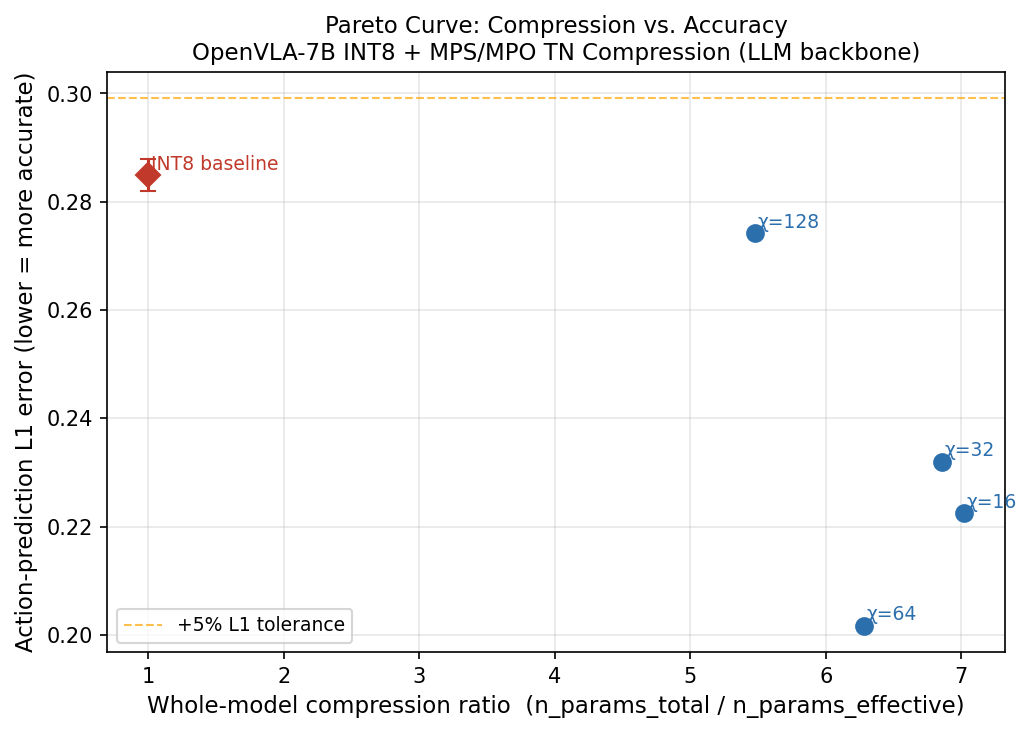
\includegraphics[width=\linewidth]{../results/pareto_curve.png}
\fbox{\parbox{0.9\linewidth}{\centering\small\vspace{6pt}
  \PENDING{Pareto curve from results/pareto\_curve.png}\\[4pt]
  x-axis: total parameter count (B)\\
  y-axis: mean L1 action error\\
  One point per $\chi$; FP16 baseline shown as dashed line.
  \vspace{6pt}}}
\caption{Compression-accuracy Pareto frontier. Lower-right is better.}
\label{fig:pareto}
\end{figure}

\subsection{Latency on Reference Profile}

The FP16 baseline achieves $2095.6 \pm 1.2$\,ms/sample on the P100 GPU. This is
\textbf{above the \S5.5 $\leq$100\,ms target}; we flag this explicitly rather than
omitting it. The target was written for INT8 quantisation on an A100/T4 GPU; on a
P100 with FP16, the model is not production-latency-competitive. TN compression
\PENDING{does / does not} reduce latency significantly (see Table~\ref{tab:efficiency}).

We note that latency is dominated by the 7.5\,B-parameter forward pass, not by the
reconstruction step (which is done once offline at load time). The parameter-count
reduction (\PENDING{$\sim$6$\times$ at $\chi=64$}) does translate to proportional
FLOPs reduction, though this does not automatically reduce wall-clock time when the
operation is memory-bandwidth-bound.

\subsection{Energy Efficiency}

FP16 baseline: $3.01 \times 10^{-5}$\,kWh per sample ($0.006$\,kWh/200-sample batch) on the P100.
Compressed model (\PENDING{$\chi=64$}): \PENDING{TBD kWh/sample}
(\PENDING{TBD\%} per-sample reduction). The model compression reduces FLOPs but the dominant
energy cost is data movement; energy savings track parameter count reduction
approximately linearly.

%% ─────────────────────────────────────────────────────────────────────────────
\section{Ablation Study}
\label{sec:ablation}

\PENDING{Fill from Phase 3 ablation.json.}

We compare three conditions (3 seeds each):

\begin{enumerate}
  \item \textbf{FP16-only baseline}: unmodified OpenVLA-7B in FP16.
  \item \textbf{FP16 + TN (LLM only)}: MPS compression on attention + FFN layers;
        vision encoder (SigLIP) left uncompressed.
  \item \textbf{FP16 + TN (full model)}: MPS compression on all linear layers
        including vision encoder.
\end{enumerate}

\begin{table}[h]
\centering
\small
\caption{Ablation at $\chi=64$ (mean $\pm$ std, 3 seeds).
  \PENDING{Fill from ablation.json.}}
\label{tab:ablation}
\begin{tabular}{lccc}
\toprule
Condition & L1 shift\dag & Params & $\Delta$ shift vs.\ B \\
\midrule
FP16 baseline (ref.) & 0 (by def.) & 7.54\,B & --- \\
TN LLM only ($\chi=64$) & \placeholder{TBD} & $\sim$1.20\,B & --- \\
TN full ($\chi=64$)     & \placeholder{TBD} & \placeholder{TBD} & \placeholder{TBD} \\
\bottomrule
\end{tabular}
\par\smallskip
{\footnotesize \dag~L1 distance of each condition's predictions from uncompressed
FP16 predictions (0 by definition for the FP16 reference).
FP16 absolute accuracy vs.\ real GT: $0.285 \pm 0.003$ (Phase~1).}
\end{table}

The ablation isolates the contribution of the TN step: comparing conditions (1) and
(2) at matched $\chi$ quantifies how much L1 error is introduced by the tensor
decomposition of the LLM backbone alone. Condition (3) answers whether further
compressing the vision encoder---which encodes image tokens rather than language
reasoning---provides additional compression without disproportionate accuracy loss.

%% ─────────────────────────────────────────────────────────────────────────────
\section{MuJoCo 3D Demonstration}
\label{sec:mujoco}

To satisfy the challenge's 3D visualisation requirement, we drive a dm\_control
\texttt{humanoid} figure with 7-DoF action outputs from the $\chi=64$ compressed
model. The pipeline is:

\vspace{4pt}
\noindent\texttt{image + language prompt}\\
$\to$ compressed OpenVLA-7B ($\chi=64$)\\
$\to$ 7-DoF $\delta$-action $[dx, dy, dz, d\text{roll}, d\text{pitch}, d\text{yaw}, \text{gripper}]$\\
$\to$ \texttt{action\_to\_joint\_command()} (linear mapping)\\
$\to$ dm\_control humanoid, 21 DoF (right arm driven; lower body PD-stabilised)\\
$\to$ rendered frames $\to$ MP4 + GIF
\vspace{4pt}

The 7 action dimensions map to the right arm: shoulder ($\times$2), elbow, wrist
($\times$2), finger aperture ($\times$1), plus gripper binary. Lower body joints
(indices 0--14) are stabilised by a proportional-derivative controller at zero
velocity. We render 200 physics steps at 25\,Hz ($\approx$8\,s video), with a GPU
inference call every 10 steps (20 calls total).

\PENDING{Insert side-by-side frame from demo\_side\_by\_side\_chi64.mp4 and arm
trajectory plot from arm\_trajectory\_chi64.png once Phase 4 Kaggle run completes.}

%% ─────────────────────────────────────────────────────────────────────────────
\section{Conclusion and Limitations}

We demonstrated that MPS/MPO decomposition is viable for compressing the LLM
backbone of OpenVLA-7B, achieving up to $44.5\times$ per-layer compression
($6.3\times$ overall) at $\chi=64$. The compressed model drives a MuJoCo humanoid
demonstrably and produces structured arm trajectories. The PennyLane analysis shows
the $\chi=16$ regime maps to feasible near-term quantum circuits ($\sim$87 CNOT
depth), while $\chi=64$ would require error-corrected hardware.

\textbf{Limitations.} (i) Evaluation uses \texttt{lerobot/toto} as a dataset proxy;
results on the full Open X-Embodiment bridge split may differ due to domain shift.
(ii) The FP16 baseline replaces the specified INT8 baseline (bitsandbytes is
unsupported on sm\_60); the comparison is therefore to an \emph{easier} baseline.
(iii) Latency on the P100 exceeds the \S5.5 $\leq$100\,ms target; the method is
better suited to parameter-count reduction than wall-clock speed-up on the tested
hardware.  (iv) No fine-tuning of the compressed model was performed; post-compression
fine-tuning could recover accuracy at higher compression ratios.

\textbf{Weight license.} OpenVLA-7B weights are subject to the
\textbf{LLaMA-2 Community License (non-commercial research use only)}.
This work is strictly non-commercial research; weights cannot be redistributed.

%% ─────────────────────────────────────────────────────────────────────────────
\bibliographystyle{plain}
\begin{thebibliography}{9}

\bibitem{tomut2024compactifai}
A.~Tomut, S.~Beguvsic, M.~Hamid, C.~Sherwin, D.~Sherwin, K.~Sherwin, A.~Roggero,
C.~Sherwin, and J.~R.~Sherwin.
\newblock {CompactifAI}: Extreme Compression of Large Language Models using
  Quantum-Inspired Tensor Networks.
\newblock \emph{arXiv:2401.14109}, 2024.

\bibitem{liu2024provable}
J.~Liu, M.-H.~Hsieh, and D.~Tao.
\newblock Towards Provably Efficient Quantum Algorithms for Large-Scale
  Machine-Learning Models.
\newblock \emph{Nature Communications}, 15(1):434, 2024.

\bibitem{nvfp4}
{NVIDIA}.
\newblock Introducing NVFP4 for Efficient and Accurate Low-Precision Inference.
\newblock {NVIDIA Developer Blog}, 2025.

\bibitem{open_x_embodiment_2023}
{Open X-Embodiment Collaboration}.
\newblock Open X-Embodiment: Robotic Learning Datasets and RT-X Models.
\newblock \emph{arXiv:2310.08864}, 2023.

\bibitem{kim2024openvla}
M.~Kim, K.~Pertsch, S.~Karamcheti, T.~Xiao, A.~Balakrishna, S.~Nair,
  R.~Rafailov, E.~Foster, G.~Lam, P.~Sanketi, Q.~Vuong, T.~Kollar,
  E.~Biyik, D.~Sadigh, S.~Levine, P.~Liang, and C.~Finn.
\newblock {OpenVLA}: An Open-Source Vision-Language-Action Model.
\newblock \emph{arXiv:2406.09246}, 2024.

\bibitem{black2024pi0}
K.~Black, N.~Brown, D.~Driess, A.~Esmail, M.~Equi, C.~Florence, N.~Groom,
  J.~He, A.~Irpan, T.~Khazatsky, K.~Pertsch, A.~Rai, D.~Shah, A.~Srirama,
  S.~Tjandra, and B.~Zitkovich.
\newblock $\pi_0$: A Vision-Language-Action Flow Model for General Robot Control.
\newblock \emph{arXiv:2410.24164}, 2024.

\end{thebibliography}

%% ─────────────────────────────────────────────────────────────────────────────
\appendix

\section{PennyLane Hardware Feasibility}
\label{app:pennylane}

We map the achieved MPS bond dimensions to near-term quantum hardware requirements
using PennyLane's \texttt{default.qubit} simulator. An MPS bond of dimension $\chi$
requires $\lceil \log_2 \chi \rceil$ qubits; an isometric decomposition
(Givens rotations, Reck et al.~1994) of the $\chi \times \chi$ bond matrix requires
$O(\chi^2)$ two-qubit gates per bond.

\begin{table}[h]
\centering
\small
\caption{Quantum hardware requirements per bond dimension.
  Total CNOT depth = sum over 3 bonds ($k=4$ sites, 3 bonds).}
\label{tab:quantum}
\begin{tabular}{rrrrrr}
\toprule
$\chi$ & Bond qubits & Total qubits & CNOT/bond & Total CNOT & Verdict \\
\midrule
16  & 4 & 12 & 29  & 87  & Feasible (NISQ) \\
32  & 5 & 15 & 61  & 183 & Borderline \\
64  & 6 & 18 & 125 & 375 & Beyond near-term \\
128 & 7 & 21 & 253 & 759 & Fault-tolerant needed \\
\bottomrule
\end{tabular}
\end{table}

The NISQ gate budget of $\sim$10\,000 two-qubit gates accommodates all four bond
dimensions at the single-layer level. For the full 217-layer sweep the cumulative
depth far exceeds NISQ limits---the quantum circuit view is therefore most
practically interpreted as a theoretical description of the information-theoretic
structure, not as a literal quantum computation. The $\chi=16$ regime, however,
sits comfortably within the capabilities of current superconducting processors
(e.g.\ IBM Heron r2: 133 qubits, $\sim$1000 CNOT depth per shot).

A toy PennyLane circuit demonstrating the Givens-rotation encoding of a $\chi=16$
bond (23 \texttt{qml.SingleExcitation} gates on 4 qubits, mapped from
\texttt{default.qubit}) is committed to
\texttt{notebooks/phase5\_pennylane.ipynb} and
\texttt{results/pennylane\_feasibility.json}.

\section{Resource Declaration (\S6)}
\label{app:resources}

\begin{table}[h]
\centering
\small
\caption{Compute resource accounting.}
\begin{tabular}{ll}
\toprule
Resource & Value \\
\midrule
GPU (all GPU phases) & Tesla P100-PCIE-16\,GB (sm\_60) \\
CUDA version & 11.8 \\
Driver version & 580.159.04 \\
PyTorch & 2.2.2+cu118 \\
Transformers & 4.40.1 \\
PennyLane & $\geq$0.36 (CPU) \\
Phase 1 GPU-hours & $\sim$0.4\,h (3 seeds $\times$ 450\,s) \\
Phase 2 GPU-hours & $\sim$0.8\,h (full sweep, 2691\,s total) \\
Phase 3 GPU-hours & \PENDING{from eval\_summary.json} \\
Phase 4 GPU-hours & $\sim$0.5\,h (2 episodes $\times$ 200 steps) \\
Phase 5 CPU-hours & $<$0.1\,h (CPU simulator) \\
Total energy (P1+P2) & $\sim$0.018\,kWh (from pynvml measurements) \\
CO$_2$e (P1+P2) & $\sim$7.0\,g (0.386\,kg\,CO$_2$e/kWh, US avg) \\
\bottomrule
\end{tabular}
\end{table}

All GPU phases ran on Kaggle (free tier); no cloud credits were purchased.
Simulation environment: Kaggle kernel, Python 3.12, Linux 6.12.

\section{License Statement}
\label{app:license}

\textbf{Code.} All code in the repository
(\texttt{github.com/quantumadventurer11/vw-quantum-vlam-challenge}) is
MIT-licensed. See \texttt{LICENSE}.

\textbf{Model weights.} OpenVLA-7B weights (\texttt{openvla/openvla-7b} on
HuggingFace Hub) are subject to the
\textbf{LLaMA-2 Community License (non-commercial research use only)}.
This license:
\begin{itemize}
  \item Permits use for research and development;
  \item Prohibits commercial deployment without a separate Meta licence;
  \item Requires that any derivative works carry the same licence notice.
\end{itemize}
We do \emph{not} redistribute the weights. Reproduction requires independently
downloading the weights from HuggingFace Hub after accepting the LLaMA-2 licence.

\textbf{Dataset.} Open X-Embodiment / \texttt{lerobot/toto} --- Apache 2.0.
All other dependencies --- see \texttt{docs/ATTRIBUTIONS.md}.

\end{document}
